\cleardoublepage

\chapter{Conception de la solution}

%%%%%%%%%%%%%%%%%%%%%%%%%%%%%%%%%%%%%%%%%%%%%%%%%%%%%%%%%%%%%%%%%%%%%%%%%%%
%%%%%%%%%%%%%%%%%%%%%%%%%%%%%%%%%%%%%%%%%%%%%%%%%%%%%%%%%%%%%%%%%%%%%%%%%%%
%%%%%%%%%%%%%%%%%%%%%%%%%%%%%%%%%%%%%%%%%%%%%%%%%%%%%%%%%%%%%%%%%%%%%%%%%%%
%%%%%%%%%%%%%%%%%%%%%%%%%%%%%%%%%%%%%%%%%%%%%%%%%%%%%%%%%%%%%%%%%%%%%%%%%%%
%%%%%%%%%%%%%%%%%%%%%%%%%%%%%%%%%%%%%%%%%%%%%%%%%%%%%%%%%%%%%%%%%%%%%%%%%%%

\section{L'aspect fonctionnel}

TODO

%%%%%%%%%%%%%%%%%%%%%%%%%%%%%%%%%%%%%%%%%%%%%%%%%%%%%%%%%%%%%%%%%%%%%%%%%%%
%%%%%%%%%%%%%%%%%%%%%%%%%%%%%%%%%%%%%%%%%%%%%%%%%%%%%%%%%%%%%%%%%%%%%%%%%%%
%%%%%%%%%%%%%%%%%%%%%%%%%%%%%%%%%%%%%%%%%%%%%%%%%%%%%%%%%%%%%%%%%%%%%%%%%%%
%%%%%%%%%%%%%%%%%%%%%%%%%%%%%%%%%%%%%%%%%%%%%%%%%%%%%%%%%%%%%%%%%%%%%%%%%%%
%%%%%%%%%%%%%%%%%%%%%%%%%%%%%%%%%%%%%%%%%%%%%%%%%%%%%%%%%%%%%%%%%%%%%%%%%%%

\section{Technologies et architecture}

L'architecture d'une application est importante, car cela définie sa maintenabilité et son l'évolutivité. De plus cela permet la séparation des problèmes diminuant ainsi la complexité.

Notre application est divisée en 3 couches, appelé 3-tiers, qui est le modèle multi-tiers le plus utilisé. Cela permet de séparer le modèle de données, la partie business et l'interface de l'utilisateur. La figure \ref{architecture_3_tiers} représente la séparation de ces différentes couches. Dans cette partie je présenterai ces différentes couches, en détaillant leurs fonctions, leurs interactions et les technologies utilisées.
%\begin{figure}[!h]
%	\center
%	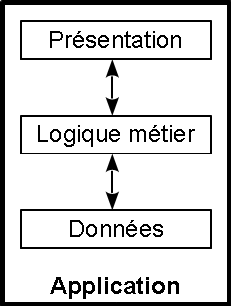
\includegraphics[width=2cm]{img/architecture_3_tiers.png}
%	\caption{Architecture 3 tiers}
%	\label{architecture_3_tiers}
%\end{figure}


%%%%%%%%%%%%%%%%%%%%%%%%%%%%%%%%%%%%%%%%%%%%%%%%%%%%%%%%%%%%%%%%%%%%%%%%%%%
%%%%%%%%%%%%%%%%%%%%%%%%%%%%%%%%%%%%%%%%%%%%%%%%%%%%%%%%%%%%%%%%%%%%%%%%%%%\\
%%%%%%%%%%%%%%%%%%%%%%%%%%%%%%%%%%%%%%%%%%%%%%%%%%%%%%%%%%%%%%%%%%%%%%%%%%%

\subsection{Socle}

La solution développée se base sur un socle existé, développé dans le cadre d'un autre projet. Ceci nous a permis un gain de temps important car une partie importante du projet n'a du être développé à nouveau.

\subsubsection{Gestion des utilisateurs}

Le socle permet une gestion des utilisateurs de l'application. Il est possible de les créer, modifier ou supprimer, pour restreindre l'accès aux personnes autorisées. De plus, il est possible de connecter l'application à un LDAP.
\\

Le \textit{LDAP}, pour Lightweight Directory Access Protocol, est un protocole standard de gestion d'utilisateurs. Son objectif est de centraliser les informations des utilisateurs (nom, identifiant, mot de passe, \ldots) dans un annuaire.

Le principal avantage de cette solution est la mise en commun des comptes utilisateurs, ce qui permet l'utilisateur d'un seul et même compte pour tous les services connectés.

TODO: schéma LDAP central et solutions connectées

\subsubsection{Gestion des droits}

Il est aussi possible de gérer des droits dans l'application grâce à ce socle. L'objectif est de contrôler les accès et les actions aux utilisateurs ayant le droit, pour protéger les informations confidentielles.
\\

Chaque écran de l'application peut avoir leur accès ou certaines actions restreintes en fonction d'un \textit{droit}. Ceux-ci peuvent prendre trois valeur : 
\begin{itemize}
  \item "aucun accès", par défaut, qui interdit tout accès à l'écran ;
  \item "lecture" n'autorise que l'accès à l'écran, avec la possibilité d'effectuer des recherches ou d'afficher les détails ;
  \item "lecture et écriture" autorise toutes les actions possibles.
\end{itemize}

Un \textit{profil} est un ensemble de droits, qui permet de définir un périmètre d'action. Par exemple un profil "administrateur" aura tous les droits dans l'application, un profil "manager" n'aura que des droits de lecture, ou encore un profil "ressource humaine" possèdera les droits liés aux candidats et contrats, \ldots

Chaque utilisateur possède un ou plusieurs profils, ce qui permet de définir l'ensemble de ses droits. L'utilisation de profils plutôt que de directement de droit permet un gain de temps, car la personne administrant les utilisateurs n'aura pas à affecter les nombreux droits aux nouveaux utilisateurs, et la modification d'un profil permet d'impacter l'ensemble des utilisateurs associés.
\\

La figure \ref{utilisateur_profils_droits} représente le schéma UML des utilisateurs, profils et droits dans l'application.
%\begin{figure}[!h]
%	\center
%	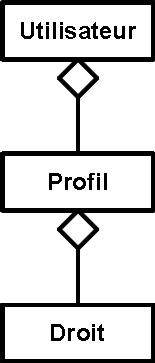
\includegraphics[width=2cm]{img/utilisateur_profils_droits.png}
%	\caption{Utilisation des profils et droits des utilisateurs}
%	\label{utilisateur_profils_droits}
%\end{figure}

%%%%%%%%%%%%%%%%%%%%%%%%%%%%%%%%%%%%%%%%%%%%%%%%%%%%%%%%%%%%%%%%%%%%%%%%%%%
%%%%%%%%%%%%%%%%%%%%%%%%%%%%%%%%%%%%%%%%%%%%%%%%%%%%%%%%%%%%%%%%%%%%%%%%%%%
%%%%%%%%%%%%%%%%%%%%%%%%%%%%%%%%%%%%%%%%%%%%%%%%%%%%%%%%%%%%%%%%%%%%%%%%%%%

\subsection{Base de données}

Une \textit{base de données} permet de stocker un grand nombre d'informations ayant des natures différentes. Ces informations sont stockées dans des tables, où les clés permettent de définir les liens de dépendant entre les informations.

%%%%%%%%%%%%%%%%%%%%%%%%%%%%%%%%%%%%%%%%%%%%%%%%%%%%%%%%%%%%%%%%%%%%%%%%%%%

\subsubsection{SQL Server 2008}

Il existe de nombreux système de gestion de base de données : Oracle, MySQL, PostgreSQL, \ldots Nous avons utilisé \textit{Microsoft SQL Server}, dans sa version 2008 R2, par demande du client.

TODO: licence : ce choix car licence déjà achetée pour d'autres ?

%%%%%%%%%%%%%%%%%%%%%%%%%%%%%%%%%%%%%%%%%%%%%%%%%%%%%%%%%%%%%%%%%%%%%%%%%%%

\subsubsection{Mapping de la base de données}

Le \textit{modèle relationnel} est utilisé dans les systèmes de gestion de base de données (SGBD) pour rassembler un ensemble d'informations. Les données (clés) sont dupliquées entre les tables et l'accès aux relations s'effectue ensuite grâce à des jointures entre les tables.

Le \textit{modèle objet}, quant à lui, est utilisé dans la programmation orientée objet. Les données sont modélisées sous la formes d'objets, entités complexes ayant des comportements et des relations entre elles.
\\

Le \textit{mapping objet-relationnel} consiste à interfacer le modèle relationnel d'une base de données avec le modèle orienté objet d'un programme informatique. Généralement, une classe modélisera une table, et attribut d'objet modélisera un champ d'une table, avec un type similaire (par exemple \lstinline{String} pour \lstinline{varchar}).
\\

Cette opération peut être faite à l'aide d'un framework (TODO: glossaire), permettent de s'abstraire de la base de données, automatisant et réduisant ainsi la duplication de code. L'objectif est de faciliter le développement, augmenter la maintenabilité du programme, ou encore s'abstenir du type de base de données.

Microsoft propose plusieurs framework, et c'est \textit{Entity Framework} qui a été utilisé. Il est intégré à Visual Studio, ce qui permet une génération et un paramétrage facilité. De plus, il permet l'interaction avec  LINQ (Language-Integrated Query), extension du langage permettant de faire des requêtes sur des ensembles de données s'abstrayant du type.

%%%%%%%%%%%%%%%%%%%%%%%%%%%%%%%%%%%%%%%%%%%%%%%%%%%%%%%%%%%%%%%%%%%%%%%%%%%
%%%%%%%%%%%%%%%%%%%%%%%%%%%%%%%%%%%%%%%%%%%%%%%%%%%%%%%%%%%%%%%%%%%%%%%%%%%
%%%%%%%%%%%%%%%%%%%%%%%%%%%%%%%%%%%%%%%%%%%%%%%%%%%%%%%%%%%%%%%%%%%%%%%%%%%

\subsection{Les services}

%%%%%%%%%%%%%%%%%%%%%%%%%%%%%%%%%%%%%%%%%%%%%%%%%%%%%%%%%%%%%%%%%%%%%%%%%%%

\subsubsection{Fonction}

La couche de \textit{service} est la partie métier de l'application. Cela permet de séparer le code source lié à l'affichage destiné à l'utilisateur, du code métier effectuant des manipulations dans la base de données.

%%%%%%%%%%%%%%%%%%%%%%%%%%%%%%%%%%%%%%%%%%%%%%%%%%%%%%%%%%%%%%%%%%%%%%%%%%%

\subsubsection{Client-Serveur}

\Jparagraph{Web service}

Un \textit{service web} (ou \textit{web service}) est un programme informatique permettant la communication et l'échange d'informations entre des systèmes hétérogènes et distribués (local, réseau, internet, \ldots), exposant ainsi des fonctionnalités.

L'échange d'informations entre le client et le serveur se fait par sérialisation, consistant à coder les informations contenues en mémoire. Cela peut se faire sous le format texte (XML, JSON, \ldots) ou au format binaire.


\Jparagraph{Windows Communication Foundation}

\textit{Windows Communication Foundation}, couramment appelé sous ses initiales WCF, est la couche de communication de .NET Framework. Cette technologie respecte les normes standards des services web, ce qui lui permet d'appeler ou d'être appelé par des technologies différentes (Java, Python, \ldots).

(TODO: aucun rapport avec WCF, mais plutôt Silverlight ?)
Les différents appels du service web se font de façon asynchrone : le client n'attend pas la réponse du serveur pour continuer son traitement. Cette solution permet de ne pas bloquer l'interface de l'utilisateur, qui pourrait penser à un plantage de l'application. Mais l'inconvénient est l'augmentation de la complexité de programmation car il est nécessaire de contrôler plusieurs fils d'exécution en parallèle.


\Jparagraph{WCF RIA Services}

Il est souvent nécessaire de posséder une logique applicative à la fois du coté serveur que du coté client. C'est le cas par exemple lorsque l'on souhaite vérifier la validité des données avant de les insérer en base de données : soit on effectue la même vérification du coté client et serveur, ce qui impose de dupliquer le code dans les deux couches, soit on n'effectue la vérification coté serveur, ce qui impose une communication inutile entre client et serveur.

Pour éviter ce problème, Microsoft propose le framework \textit{WCF RIA Services}. Cet outil génère du code, contenu du coté serveur, dans la couche client, lors de la compilation.
\\


La figure \ref{WCF_RIA_Services} représente les échanges entre la partie cliente de l'application et la partie serveur.
%\begin{figure}[!h]
%	\center
%	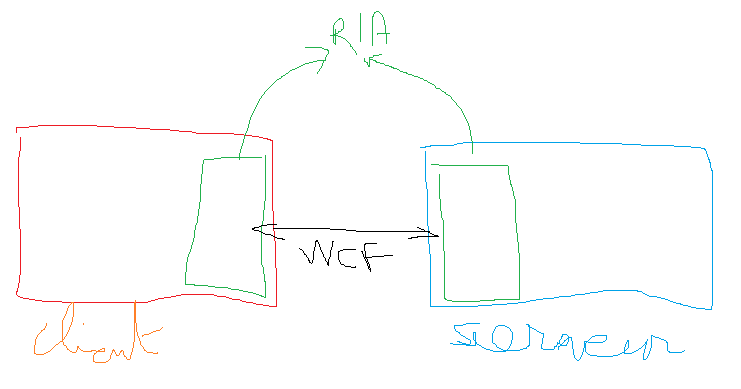
\includegraphics[width=2cm]{img/WCF_RIA_Services.png}
%	\caption{Fonctionnement de l'application client-serveur}
%	\label{WCF_RIA_Services}
%\end{figure}

%%%%%%%%%%%%%%%%%%%%%%%%%%%%%%%%%%%%%%%%%%%%%%%%%%%%%%%%%%%%%%%%%%%%%%%%%%%
%%%%%%%%%%%%%%%%%%%%%%%%%%%%%%%%%%%%%%%%%%%%%%%%%%%%%%%%%%%%%%%%%%%%%%%%%%%
%%%%%%%%%%%%%%%%%%%%%%%%%%%%%%%%%%%%%%%%%%%%%%%%%%%%%%%%%%%%%%%%%%%%%%%%%%%

\subsection{Interface utilisateur}

\subsubsection{Silverlight}

Microsoft \textit{Silverlight} est un plugin pour navigateur web, permettant le développement d'applications riches. Le but est de pousser plus loin l'expérience utilisateur du web 2.0. Initialement prévu pour fonctionner dans un navigateur, les programmes peuvent être installés directement sur l'ordinateur ("out of browser"), et permettent de développer des application pour Windows Phone 7.

Cette technologie nécessite l'installation du plugin, qui est un sous-ensemble de Microsoft .NET Framework. L'avantage est d'être cross-browser (Internet Explorer, Firefox, Chrome, \ldots) et cross-platform (Windows, OS-X et Linux, via le projet open-source Moonlight). Les applications fonctionnent donc dans une "sandbox" (bac a sable) qui permet de garantir une sécurité pour l'utilisateur et le serveur.







-----------------------------------------



Le groupe Limagrain travaille dans un environnement Micosoft et utilise ainsi leurs technologies et logiciels, comme par exemple : Windows, Internet Explorer, Outlook, etc.

Pour développer cette solution nous nous sommes donc tourné vers les technologies Microsoft pour faciliter la compatibilité et l'intégration des composants.

%%%%%%%%%%%%%%%%%%%%%%%%%%%%%%%%%%%%%%%%%%%%%%%%%%%%%%%%%%%%%%%%%%%%%%%%%%%
%%%%%%%%%%%%%%%%%%%%%%%%%%%%%%%%%%%%%%%%%%%%%%%%%%%%%%%%%%%%%%%%%%%%%%%%%%%
%%%%%%%%%%%%%%%%%%%%%%%%%%%%%%%%%%%%%%%%%%%%%%%%%%%%%%%%%%%%%%%%%%%%%%%%%%%

\subsection{Langage de programmation}

\textit{.NET} est une plateforme application proposée par Microsoft. Cette technologie est comparable et directement concurrente de Java d'Oracle.

Ce framework propose de nombreux composants :
\begin{enumerate}
\item Plusieurs environnements d'exécution. Un moteur d'exécution permettant la compilation du code source, et qui sera à son tour compilé "à la volée" pour être exécuté dans la machine virtuelle. Un environnement d'exécution de services et d'applications web, appelé ASP .NET. Et enfin un environnement d'exécution d'applications lourdes, appelé WinForms.
\item Un kit de développement, aussi appelé Software Development Kit (SDK), fournissant une bibliothèque de classes aux développeurs.
\end{enumerate}



La solution sera développée dans un langage Microsoft
